\documentclass[twocolumn]{article}
\usepackage{authblk}
\usepackage{times}
\usepackage{graphicx}
\usepackage{float}
\usepackage{gensymb}
\usepackage{siunitx}
\graphicspath{ {../Plots/} }
\title{EPR Fitting of an Unknown Substance Using EasySpin}
\author{Patrick McMillin}
\affil{Department of Physics and Astronomy, California State University Northridge}
\date{8 March 2018}
\begin{document}
% need this to get the abstract centered 
\twocolumn[
	\begin{@twocolumnfalse}
		\maketitle
		\begin{abstract}
		Electron paramagnetic resonance (EPR) spectroscopy allows us to gain valuable dynamical information from systems of molecules. From experimentally collected EPR data of an unknown substance at temperatures between 20 $\degree$C and 100 $\degree$C, we employed the MATLAB fitting software EasySpin to obtain information about the hyperfine interactions, g-factor, and the rotational diffusion of the system. We find there is no relationship between temperature and the $g$-factor, and a positive relationship between temperature and the hyperfine interactions. Finally, we observe an Arrhenius relationship between the temperature and the rotational correlation times $\tau$.
		\end{abstract}
	\end{@twocolumnfalse}
] % ending this makes it two column again
\section{Introduction}
\label{sec:introduction}
Electron paramagnetic resonance (EPR) spectroscopy uses the Zeeman effect to gather photon absorption data from a system which is subject to an external magnetic field. Additional theory is presented in Section~\ref{sec:theory}.\\
\indent
We will look specifically at three properties obtained from fitting the spectra: the $g$-factor, the strength of the hyperfine interactions, and the rotational correlation times. These three properties will allow us to draw conclusions about our unknown substance and its dynamics. 
\section{Theory}
\label{sec:theory}
The applied magnetic field $B$ causes the unpaired electrons in the system to occupy one of two available states based on their intrinsic spin. These states are either aligned in parallel or antiparallel with the direction of $B$. The energy difference of these states is given by equation \ref{eq:1}.
\begin{equation} 
\Delta E = g\mu_BB
\label{eq:1}
\end{equation}
Where $g$ is the $g$-factor, $\mu_B$ is the Bohr magneton, and $B$ is the external magnetic field. \\
Switching energy levels requires photon emission or absorption, which is facilitated by applying an external beam of light to be applied to the sample. The energy-frequency relation of photons is given by equation \ref{eq:2}.
\begin{equation}
\Delta E=h\nu
\label{eq:2}
\end{equation}
Where $h$ is Planck's constant (6.626$\times$10$^{-34}$\si{J.s}), and $\nu$ is the frequency of the photon. \\
\subsection{The $g$-factor}
The $g$-factor is a value which serves in several ways as a 'fingerprint' of the system, as the spectra will peak when the the magnetic field is tuned to such a value that causes the energy difference to match that of the applied light source.\\
\indent
The parameters produced by the line fitting give us the diagonal elements of the $g$-factor tensor. We are interested in the isotropic value of $g$, given by equation \ref{eq:3}.
\begin{equation}
g_{iso}=\frac{g_{xx}+g_{yy}+g_{zz}}{3}
\label{eq:3}
\end{equation}
Where $g_{xx}$, $g_{yy}$, and $g_{zz}$ correspond to the first, second, and third diagonal elements of the $g$ tensor respectively. 
\\
\subsection{The Hyperfine Interaction}
The hyperfine interaction strength or $A$ value gives us useful information about the structure of the system we consider. The surrounding atoms which have spin will induce localized magnetic fields at the area of the unpaired electrons. This interaction is called the hyperfine interaction, and serves as a molecular measurement tool. Additionally, the strength of this interaction tells us about the composition of the nearby atoms. The hyperfine interaction manifests itself in the spectra by splitting the lines observed due to the material's $g$-factor. The number of lines in the spectra can be given by equation \ref{eq:4}.
\begin{equation}
\text{Number of Lines} = 2nI+1
\label{eq:4}
\end{equation}
Where n is the number of nuclei present, and I is the spin of the nucleus. The strength of the hyperfine interaction is captured through the distance between the split spectral lines. A weak hyperfine interaction (from a distant nucleus) will cause lines to be further apart. \\
\indent
The parameters produced by the line fitting give us the diagonal elements of the $A$ tensor. We are interested in the isotropic value of $A$, given by equation \ref{eq:5}.
\begin{equation}
A_{iso}=\frac{A_{xx}+A_{yy}+A_{zz}}{3}
\label{eq:5}
\end{equation}
Where $A_{xx}$, $A_{yy}$, and $A_{zz}$ are given by the first, second, and third diagonal elements of the $A$ tensor. 
\subsection{Rotational Correlation Time}
The rotational correlation time is captured by the width and shape of the spectral lines. Broadened lines correspond to very fast correlation times, where sharp lines indicate a slow correlation time. This means that a freely moving molecule will produce sharp lines, and a relatively localized molecule will produce broad lines. \\
\indent
From the fitting program, we are given the logarithm of the diffusion, and can find the correlation time by using equation \ref{eq:6}.
\begin{equation}
\tau = \frac{10^{-\tau_{R}}}{6}10^9\si{ns}
\label{eq:6}
\end{equation}
Where $\tau$ is the rotational correlation time, and $\tau_{R}$ is the diffusion. 
\section{Methods}
\label{sec:methods}
We were given seventeen experimental EPR spectra of an unknown substance, each spectra had a known temperature between 20 $\degree$C and 100 $\degree$C in intervals of 5 $\degree$C. The spectra were given to us in arbitrary units of intensity (A.U.) versus the magnetic field strength $B$ in Gauss. \\
\subsection{Fitting with EasySpin}
Through the use of the MATLAB based program EasySpin, we used a pre-written fitting script to fit all of the seventeen spectra. With careful initial guesses, the program can fit a theoretical curve to the experimental spectrum using the Levenberg/Marquardt fitting method to find the best fit. The fitting gives the user the decomposed components of the g-factor, the hyperfine interaction strength, and the log of the correlation time. All of these parameters were exported and placed in a data file in order to complete calculations of the isometric g-factor, the isometric hyperfine interaction strength, and the rotational correlation time. \\
\indent
Fifteen of the seventeen spectra were fitted properly. The spectra for the 20 $\degree$C and 45 $\degree$C were not fitted properly, and thus they were excluded from this study. \\
\indent
After fitting, the MATLAB program displays a plot which contains the experimental spectrum, the fitted curve, and a line which shows the difference between the fitted curve and the experimental spectrum. This plot can be seen in Figure  \ref{fig:fig1} for the system at 80 $\degree$C.
\begin{figure}[h]
	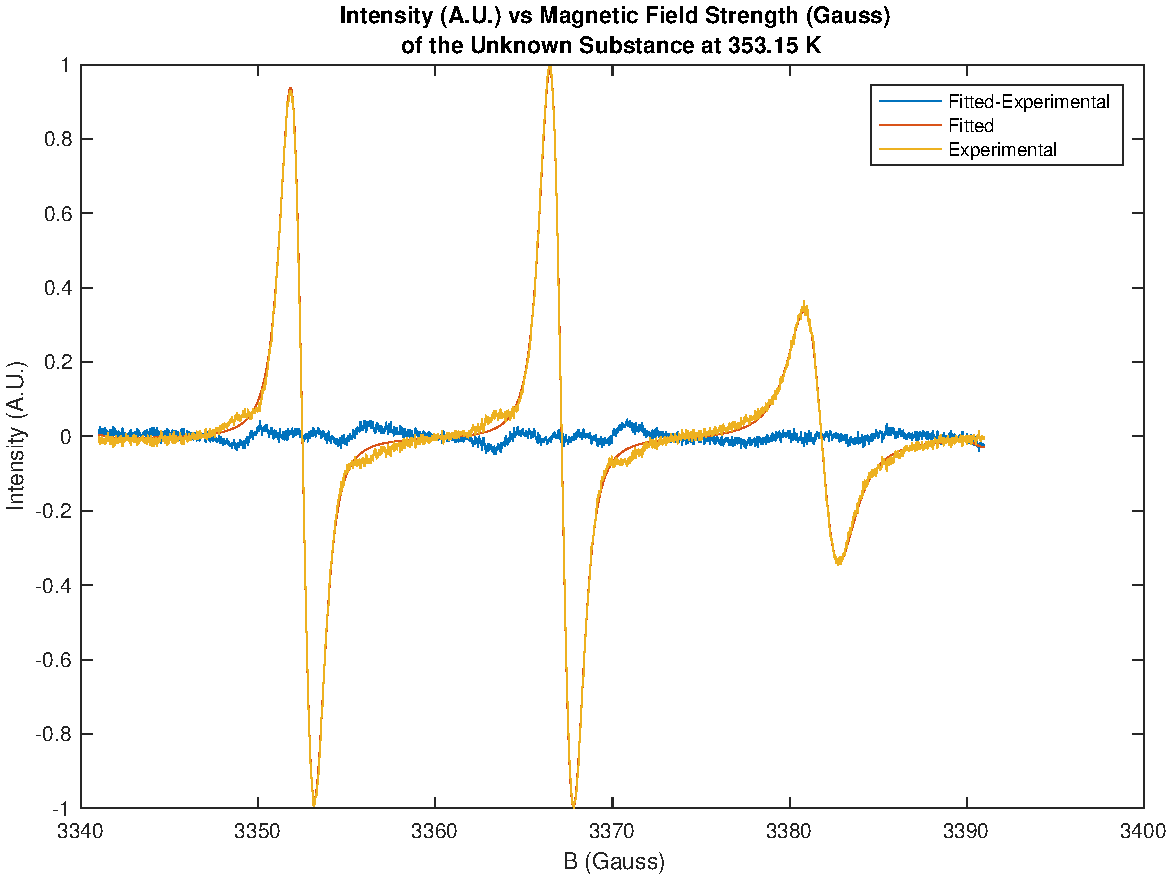
\includegraphics[scale=0.35]{H80C1_Best_Fit_for_Report_try}
	\caption{Plot of the experimentally obtained spectrum, the EasySpin fitted line, and the difference between the fitted line and the experimental spectrum.\label{fig:fig1}}
\end{figure}
\subsection{Analysis of the Fitting}
The analysis of the results was performed through a home-made python script after exporting all of the necessary data to a text file. 
\indent
The plots of $g_{iso}$ versus temperature and $A_{iso}$ versus temperature (figures \ref{fig:fig2} and \ref{fig:fig3}, respectively) were both fitted by a simple line (equation \ref{eq:7}). 
\begin{equation}
y=mx+b
\label{eq:7}
\end{equation}
The plot of the rotational correlation time $\tau$ was fitted by the Arrhenius equation (equation \ref{eq:8}). 
\begin{equation}
\tau=\tau_0e^{\frac{-x}{R(T-T_0)}}
\label{eq:8}
\end{equation}
Where $\tau$ is the rotational correlation time, $\tau_0$ is a scaling factor with units in \si{ns}, $x$ is the activation energy of the molecule in Joules, $T$ is the temperature of the system in Kelvin, $R$ is the universal gas constant (8.314 \si{J.mol^{-1}.K^{-1}}, and $T_0$ is a reference temperature in Kelvin.
\section{Results and Discussion}
\label{sec:results}
\subsection{The $g$-factor of the Unknown Substance}
\label{sec:Resultsgfact}
After fitting a simple line (equation \ref{eq:7}) to the experimentally obtained $g_{iso}$ values as a function of temperature through a chi=squared minimization procedure, the fitting parameters $m$ and $b$ (slope and $y$-intercept) were found to be $m=-2.418\times 10^{-6}$ and $b=2.006$. This tells us that the $g_{iso}$ value is approximately 2.006 which only changes with 2 parts per million per Kelvin. The plot of the $g_{iso}$ values as a function of temperature can be found in figure \ref{fig:fig2}. The $g_{iso}$ value of approximately 2 tells us that we are dealing with unpaired electrons in our substance, which is certainly expected. 
\begin{figure}[h]
	\includegraphics[scale=0.49]{g_iso_Plot}
	\caption{Plot of the $g$-factor versus temperature (\si{K}). The red dots are the $g_{iso}$ values obtained from fitting with EasySpin, and the blue line is the fitted line form the home-made analysis script. The fitted line is discussed in section \ref{sec:Resultsgfact}.\label{fig:fig2}}
\end{figure}
\subsection{Hyperfine Interactions of the Unknown Substance}
\label{sec:ResultsAfact}
\begin{figure}[H]
	\includegraphics[scale=0.49]{A_iso_Plot}
	\caption{Plot of the hyperfine interaction strength $A_{iso}$ versus temperature (\si{K}). The red dots are the $A_{iso}$ values obtained from fitting with EasySpin, and the blue line is the fitted line form the home-made analysis script. The fitted line is discussed in section \ref{sec:ResultsAfact}.\label{fig:fig3}}
\end{figure}
Fitting of the $A_{iso}$ value was very similar to that of $g_{iso}$. Fitting to a simple line through a chi-squared minimization process produced the values $m=4.68\times 10^{-3}$ and $b=39.8$. These values tell us that although $A_iso$ does not change much in temperature per Kelvin, there still is a noticeable slope throughout our target range of 293 \si{K} to 373 \si{K}. The plot of the $A_{iso}$ values as a function of temperature can be found in figure \ref{fig:fig3}. The strength of the hyperfine interactions increases with temperature, which can be concluded from the positive value of $m$. 
\subsection{Rotational Correlation Times of the Unknown Substance}
\label{sec:ResultsRotCorr}
Fitting of the rotational correlation time $\tau$ was done through a chi-squared minimization process by using equation \ref{eq:8}. Fitting this equation gives us the Arrhenius activation energy in the form of $x$. The fitting gave us values of $\tau_{0}=2.79\times 10^{-5}$, $T_0=77.9$, and $x=-23060$  \si{J}. This $x$ value can be written instead as -5.51 \si{kcal.mol^{-1}}, which is the activation energy of the substance. 
\begin{figure}[h]
	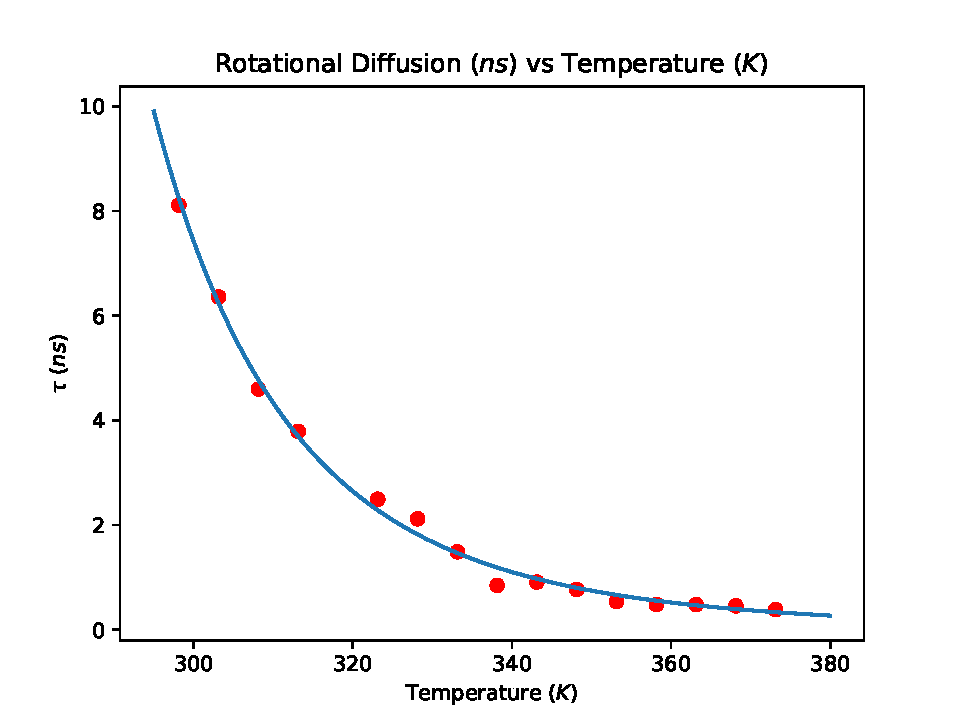
\includegraphics[scale=0.49]{Rot_Dif_plot}
	\caption{Plot of the rotational correlation time $\tau$ versus temperature (\si{K}). The red dots are values obtained from the EasySpin fitting after having equation \ref{eq:6} applied to them. The fitted line is discussed in section \ref{sec:ResultsRotCorr}.\label{fig:fig4}}
\end{figure}
\section{Conclusions}
\label{sec:conclusions}
From our fitted data, we see that the value of $g_{iso}$ is constant in temperature, as expected. Additionally, we find that there is a positive linear relationship between temperature and the $A_{iso}$ value. Finally, we see an appropriate Arrhenius relationship between the temperature and the rotational correlation time $\tau$. From a fitting, we find that the activation energy of the unknown substance is -5.51 \si{kcal.mol^{-1}}. The fitting process that I employed is not perfect, and in the future I will attempt to fit more properly. 
\section{References}
\label{sec:references}
-An EPR Primer. (n.d.). Retrieved March 7, 2018.
Retrieved form the PHYS 466 Canvas page.\\
-Griffiths, D. J. (2017). Introduction to Quantum Mechanics. New York, NY: Cambridge. \\
-Schroeder, D. V. (2000). An Introduction to Thermal Physics. San Francisco, CA. Addison Wesley Longman.
\end{document}
